%!TEX root =../quadrotorbook.tex
\chapter{Trajectory Generation and Local Planning}
\label{chap:trajectory_planning}

The objective of this chapter is to plan trajectories through a map that represents a cluttered world environment.  The high-level architecture for this chapter is shown in Figure~\ref{fig:planning_architecture}.
\begin{marginfigure}[3in]
  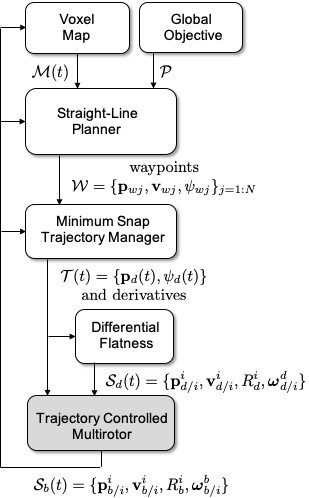
\includegraphics[width=\linewidth]{chap5_trajectory_planning/figures/planning_architecture}
  \caption{The path planning architecture outlined in this chapter.}
  \label{fig:planning_architecture}  
\end{marginfigure}
At the highest level is a voxel representation of the world, local the the multirotor.  The voxel grid will evolve dynamically so that the multirotor always remains in voxel at the center of the map.  A straight-line path planner is then used to plan paths through the voxel map that minimize the distance to the goal location as well as minimize the associated risk.  The output of the straight-line planner is a set of waypoints $\mathcal{W}$ specified as a sequence of desired positions, desired velocities, and desired heading directions.  The waypoints are processed by the {\em minimum-snap trajectory} block to produce a time trajectory of position and heading where the fourth derivative (snap) of the position trajectory is minimized.  The trajectory can be fed directly into the trajectory following framework discussed in Chapter~\ref{chap:trajectory_following}.  However, the framework in Chapter~\ref{chap:trajectory_following} also requires velocity, and angular velocity of the desired multirotor frame.  Those elements are naturally produced by the {\em differential flatness} block shown in Figure~\ref{fig:planning_architecture}.


%----------------------------------
\section{Differential Flatness}
\label{sec:differential_flatness}

Consider the nonlinear system
\begin{equation}\label{eq:flat-system}
\dot{x} = f(x,u),
\end{equation}
where $x$ is the state and $u\in\mathbb{R}^m$ is the control input, and the output mapping
\begin{equation}\label{eq:flat-output}
z = h(x),
\end{equation}
where $z\in\re^p$.  We say that the system~\eqref{eq:flat-system} is differentially flat with flat output $z$ if the following conditions hold~\cite{CowlingYakimenkoWhidborne07}:
\begin{enumerate}
\item The components of $z$ are not differentially related over time.
\item The states $x$ can be written as a function of the flat output and its derivatives, i.e., there exists a function $g_1$, and a finite scalar $m_1$ such that
    \begin{equation}\label{eq:flat-g1}
    x(t) = g_1\left(z(t),\frac{d}{dt}z(t),\cdots,\frac{d^{m_1}}{dt^{m_1}}z(t)\right).
    \end{equation}
\item The control inputs $u$ can be written as a function of the flat output and its derivatives, i.e., there exists a function $g_2$ and a finite scalar $m_2$ such that
    \begin{equation}\label{eq:flat-g2}
    u(t) = g_2\left(z(t),\frac{d}{dt}z(t),\cdots,\frac{d^{m_2}}{dt^{m_2}}z(t)\right).
    \end{equation}
\end{enumerate}

We now show that the multi-rotor system is differentially flat.

\begin{theorem}[Multirotor is Differentially Flat]

Suppose that the multirotor system is given by
\begin{align}
\dot{\pbf}_{d/i}^i &= \vbf_{d/i}^i \label{eq:flat-multirotor-1} \\
\dot{\vbf}_{d/i}^i &= g \ebf_3 + T_d R_d^i \ebf_3 \label{eq:flat-multirotor-2} \\
\dot{R}_d^i &= R_d^i \ss{\omegabf_{d/i}^d}, \label{eq:flat-multirotor-3}
\end{align}
and let $\psi$ be the heading angle, i.e., the body $x$-axis projected onto the inertial $x-y$ plane is 
$\sbf_\psi\doteq (\cos\psi, \sin\psi, 0)^\top$.  

Then the multirotor system is differentially flat with flat outputs $\{\pbf_d(t), \psi_d(t)\} \in\mathbb{R}^3 \times \mathbb{R}$.
\end{theorem}
\begin{proof}
To show that the system is differentially flat, the state variables $\pbf_{d/i}^i$, $\vbf_{d/i}^i$, $R_d^i$ and the input variables $T_d$ and $\omegabf_{d/i}^d$ must all be expressed in terms of the flat outputs $\{\pbf_d(t), \psi_d(t)\}$ and their derivatives.

The position states are directly expressed in the flat outputs as $\pbf_{d/i}^i = \pbf_d(t)$.  The velocity states are directly expressed in the derivative of the flat outputs as $\vbf_{d/i}^i = \dot{\pbf}_d(t)$.

Let the rotation matrix be expressed as 
\[
R_d^i = \begin{pmatrix} \rbf_{1d} & \rbf_{2d} & \rbf_{3d} \end{pmatrix},
\]
where $r_{jd}$ is the $j^{th}$ desired body axis of the multirotor expressed in the inertial frame. Therefore Equation~\eqref{eq:flat-multirotor-2} becomes
\[
T_d r_{3d} = \dot{\vbf}_{d/i}^i - g \ebf_3,
\]
which implies that 
\begin{align*}
T_d &= \norm{\dot{\vbf}_{d/i}^i - g \ebf_3^i} \\
\rbf_{3d} &= \frac{\dot{\vbf}_{d/i}^i - g \ebf_3}{\norm{\dot{\vbf}_{d/i}^i - g \ebf_3}}.
\end{align*}
Therefore the input $T_d$ and the third row of the rotation matrix can be expressed in terms of the flat output as
\begin{align*}
T_d &= \norm{\ddot{\pbf}_d - g \ebf_3} \\
\rbf_{3d} &= \frac{\ddot{\pbf}_d - g \ebf_3}{\norm{\ddot{\pbf}_d- g \ebf_3}}.
\end{align*}
The cross product between the body frame $z$-axis $\rbf_{3d}$ and the heading vector $\sbf_{\psi_d}$ will be in the direction of the body frame $y$-axis and should always be in the inertial $x-y$ plane.  Therefore, $\rbf_{2d}$ is expressed in terms of the flat outputs as
\[
\rbf_{2d} = \frac{\rbf_{3d} \times \sbf_{\psi_d}}{\norm{\rbf_{3d} \times \sbf_{\psi_d}}}.
\]
Since the body frame is a right-handed coordinate system, the body $x$-axis is given by
\[
\rbf_{1d} = \rbf_{2d} \times \rbf_{3d}.
\]
We have shown that $R_d^i$ can be expressed in terms of $\dot{\pbf}_d$ and $\psi_d$.  By differentiating $R_d^i$ it is clear that $\dot{R}_d^i$ can be expressed in terms of $\dot{\pbf}_d$, $\ddot{\pbf}_d$, $\psi_d$ and $\dot{\psi}_d$.  

From Equation~\eqref{eq:flat-multirotor-3}, the angular velocity vector is given by
\[
\omegabf_{d/i}^d = \left(R_d^{i\top} \dot{R}_d^i\right)^\vee. 
\]

Summarizing, the states and outputs are expressed in the flat outputs and their derivatives as
\begin{align*}
\pbf_{d/i}^i(\pbf_d) &= \pbf_d(t) \\
\vbf_{d/i}^i(\dot{\pbf}_d) &= \dot{\pbf}_d(t) \\
\rbf_{3d}(\ddot{\pbf}_d) &= \frac{\ddot{\pbf}_d - g \ebf_3}{\norm{\ddot{\pbf}_d - g \ebf_3}} \\
\rbf_{2d}(\ddot{\pbf}_d, \psi_d) &= \frac{\rbf_{3d} \times \sbf_{\psi_d}}{\norm{\rbf_{3d} \times \sbf_{\psi_d}}} \\
\rbf_{1d}(\ddot{\pbf}_d, \psi_d) &= \rbf_{2d} \times \rbf_{3d} \\
R_d^i(\ddot{\pbf}_d, \psi_d) &= \begin{pmatrix} \rbf_{1d} & \rbf_{2d} & \rbf_{3d} \end{pmatrix} \\
T_d(\ddot{\pbf}_d) &= \norm{\ddot{\pbf}_d - g \ebf_3} \\	
\omegabf_{d/i}^d(\ddot{\pbf}_d, \dddot{\pbf}_d, \psi_d, \dot{\psi}_d) &= (R_d^{i\top}\dot{R}_d^i)^\vee.
\end{align*}

Since all states and inputs can be expressed in terms of the flat outputs and their derivatives, the system is differentially flat.
\end{proof}

%++++++++++++++++++++++++++++++++++++++++++++++++++++++++++++++
\subsection{Analytic calculation of desired angular velocity}
Author: Jacob Willis

%
%\usepackage[utf8]{inputenc}
%\usepackage{amsmath}
%\usepackage{amssymb}
%\usepackage{graphicx}
%\graphicspath{ {./figs/} }
%
%% \usepackage{theorem}
%\usepackage{amsthm}
%\newtheorem{theorem}{Theorem}
%\newtheorem{property}{Property}
%\def\proof{\hspace{1em}{\it Proof: }}
%\def\endproof{\hspace*{\fill}~$\blacksquare$\par\endtrivlist\unskip}
%
%\newtheorem*{remark}{Remark}
%
%\usepackage[hidelinks]{hyperref}
%\usepackage{color}
%\newcommand{\rwbcomment}[1]{{\color{red} RWB: #1}}
%\newcommand{\jbwcomment}[1]{{\color{blue} JBW: #1}}
%%\usepackage{cite}
%\usepackage{multirow}
%\usepackage[margin=1in]{geometry}
%
%\usepackage{biblatex}
%\addbibresource{bib_willis/references.bib}
%
%%\DeclareMathOperator{\mod}{mod}
%\DeclareMathOperator{\floor}{floor}
%\DeclareMathOperator{\rank}{rank}
%\DeclareMathOperator{\vspan}{span}
%\DeclareMathOperator*{\argmin}{arg min}
%
%\title{\LARGE Analytic Derivative of the Desired Rotation Matrix for Control}
%\author{Jacob Willis}
%
%\begin{document}
%\maketitle

Rather than numerically differentiating $R_d^i$ as described in Section~\ref{sec:numerical_differentiation_of_R}, this section shows how to find the time derivative of $R_d^i$ analytically.
First, recall that
\begin{equation}
	R_d^i = \begin{pmatrix} \mathbf{r}_{1d} & \mathbf{r}_{2d}&  \mathbf{r}_{3d} \end{pmatrix}
\end{equation}
and therefore that
\begin{equation}
	\dot{R}_d^i = \begin{pmatrix} \dot{\mathbf{r}}_{1d} & \dot{\mathbf{r}}_{2d} & \dot{\mathbf{r}}_{3d} \end{pmatrix}.
\end{equation}

To proceed, we need the following two properties.
\begin{property}
	The time derivative of the cross product of two time-dependent vectors $\mathbf{x}$ and $\mathbf{y}$ is
	\begin{equation}
		\label{eq:cross_derivative}
		\frac{d}{dt} (\mathbf{x} \times \mathbf{y}) = \dot{\mathbf{x}} \times \mathbf{y} + \mathbf{x} \times \dot{\mathbf{y}}
	\end{equation}
\end{property}
\proof
This is easiest to see by recalling that $\mathbf{x} \times \mathbf{y} = \mathbf{x}^\wedge \mathbf{y}$ where the result follows from the product rule.
\endproof

\begin{property} \label{prop:derivative_of_normal_vector}
	The time derivative of a normalized vector $\frac{\mathbf{x}}{\|\mathbf{x}\|}$ is
	\begin{equation}
		\label{eq:norm_derivative}
		\frac{d}{dt} \left(\frac{\xbf}{\norm{\xbf}}\right) = \Pi_{\frac{\xbf}{\norm{\xbf}}} \frac{\dot{\xbf}}{\norm{\xbf}},
	\end{equation}
	where $\Pi_{\nbf} \doteq I-\nbf\nbf^\top$ is the projection operator on to the plane orthogonal to the unit vector $\nbf$.
\end{property}
\proof
	By the quotient rule, we have
	\begin{equation}
		\frac{d}{dt} \frac{\mathbf{x}}{\|\mathbf{x}\|} = \frac{\dot{\mathbf{x}} \|\mathbf{x}\| - \mathbf{x} \frac{d}{dt}(\|\mathbf{x}\|)}{\|\mathbf{x}\|^2}.
	\end{equation}
	Now,
	\begin{align}
		\frac{d}{dt} \|\mathbf{x}\| 
		= \frac{d}{dt} \sqrt{\mathbf{x}^\top \mathbf{x}} 
		= \frac{1}{2 \sqrt{\mathbf{x}^\top \mathbf{x}}} (\dot{\mathbf{x}}^\top \mathbf{x} + \mathbf{x}^\top \dot{\mathbf{x}})
		= \frac{\dot{\mathbf{x}}^\top \mathbf{x}}{\|\mathbf{x}\|}
	\end{align}
	Plugging in, we get
	\begin{equation}
		\frac{d}{dt} \frac{\mathbf{x}}{\|\mathbf{x}\|} = \frac{\dot{\mathbf{x}}}{\|\mathbf{x}\|} - \mathbf{x} \frac{\dot{\mathbf{x}}^\top \mathbf{x}}{\|\mathbf{x}\|^3}.
	\end{equation}
	Rearranging gives
	\[
	\frac{d}{dt} \frac{\mathbf{x}}{\|\mathbf{x}\|} =  \left(I-\frac{\xbf}{\norm{\xbf}}\frac{\xbf^\top}{\norm{\xbf}}\right)\frac{\dot{\xbf}}{\norm{\xbf}}.
	\]

\endproof

The third column of the rotation matrix is given by
\begin{equation}
	\mathbf{r}_{3d} = - \frac{\ddot{\mathbf{p}}_d - g \mathbf{e}_3 - K_p \tilde{\mathbf{p}} - K_d \dot{\tilde{\mathbf{p}}}} {\norm{\ddot{\pbf}_d - g \ebf_3 - K_p \tilde{\pbf} - K_d \dot{\tilde{\pbf}}}}.
\end{equation}
Therefore, using the properties above we get that
\[
\dot{\rbf}_{3d} = \Pi_{\rbf_{3d}} \left(\frac{-\dddot{\pbf}_d + K_p \dot{\tilde{\pbf}} + K_d \ddot{\tilde{\pbf}}}{\norm{\ddot{\pbf}_d - g \ebf_3 - K_p \tilde{\pbf} - K_d \dot{\tilde{\pbf}}}}\right).
\]
The second column of the rotation matrix is given by
\[
\rbf_{2d} = \frac{\rbf_{3d}\times\sbf_{\psi_d}}{\norm{\rbf_{3d}\times\sbf_{\psi_d}}},
\]
which implies that
\[
\dot{\rbf}_{2d} = \Pi_{\rbf_{2d}}\left(\frac{\dot{\rbf}_{3d}\times\sbf_{\psi_d}+\dot{\psi}_d\rbf_{3d}\times (-\sin\psi_d,  \cos\psi_d, 0)^\top }{\norm{\rbf_{3d}\times\sbf_{\psi_d}}}\right).
\]
The first column of the rotation matrix is given by
\[
\rbf_{1d} = \rbf_{2d}\times\rbf_{3d},
\]
which implies that
\[
\dot{\rbf}_{1d} = \dot{\rbf}_{2d}\times\rbf_{3d} + \rbf_{2d}\times \dot{\rbf}_{3d}.
\]
The angular velocity can now be calculated as
\[
\omegabf_{d/i}^d(\pbf_d, \dot{\pbf}_d, \ddot{\pbf}_d, \dddot{\pbf}_d, \psi_d, \dot{\psi}_d) = \left[\begin{pmatrix}\rbf_{1d} & \rbf_{2d} & \rbf_{3d}\end{pmatrix}^\top \begin{pmatrix} \dot{\rbf}_{1d} & \dot{\rbf}_{2d} & \dot{\rbf}_{3d} \end{pmatrix}\right]^\vee.
\]

\subsection{Differential Flatness of Quadrotor Dynamics Subject to Rotor Drag, RAL, 2018}
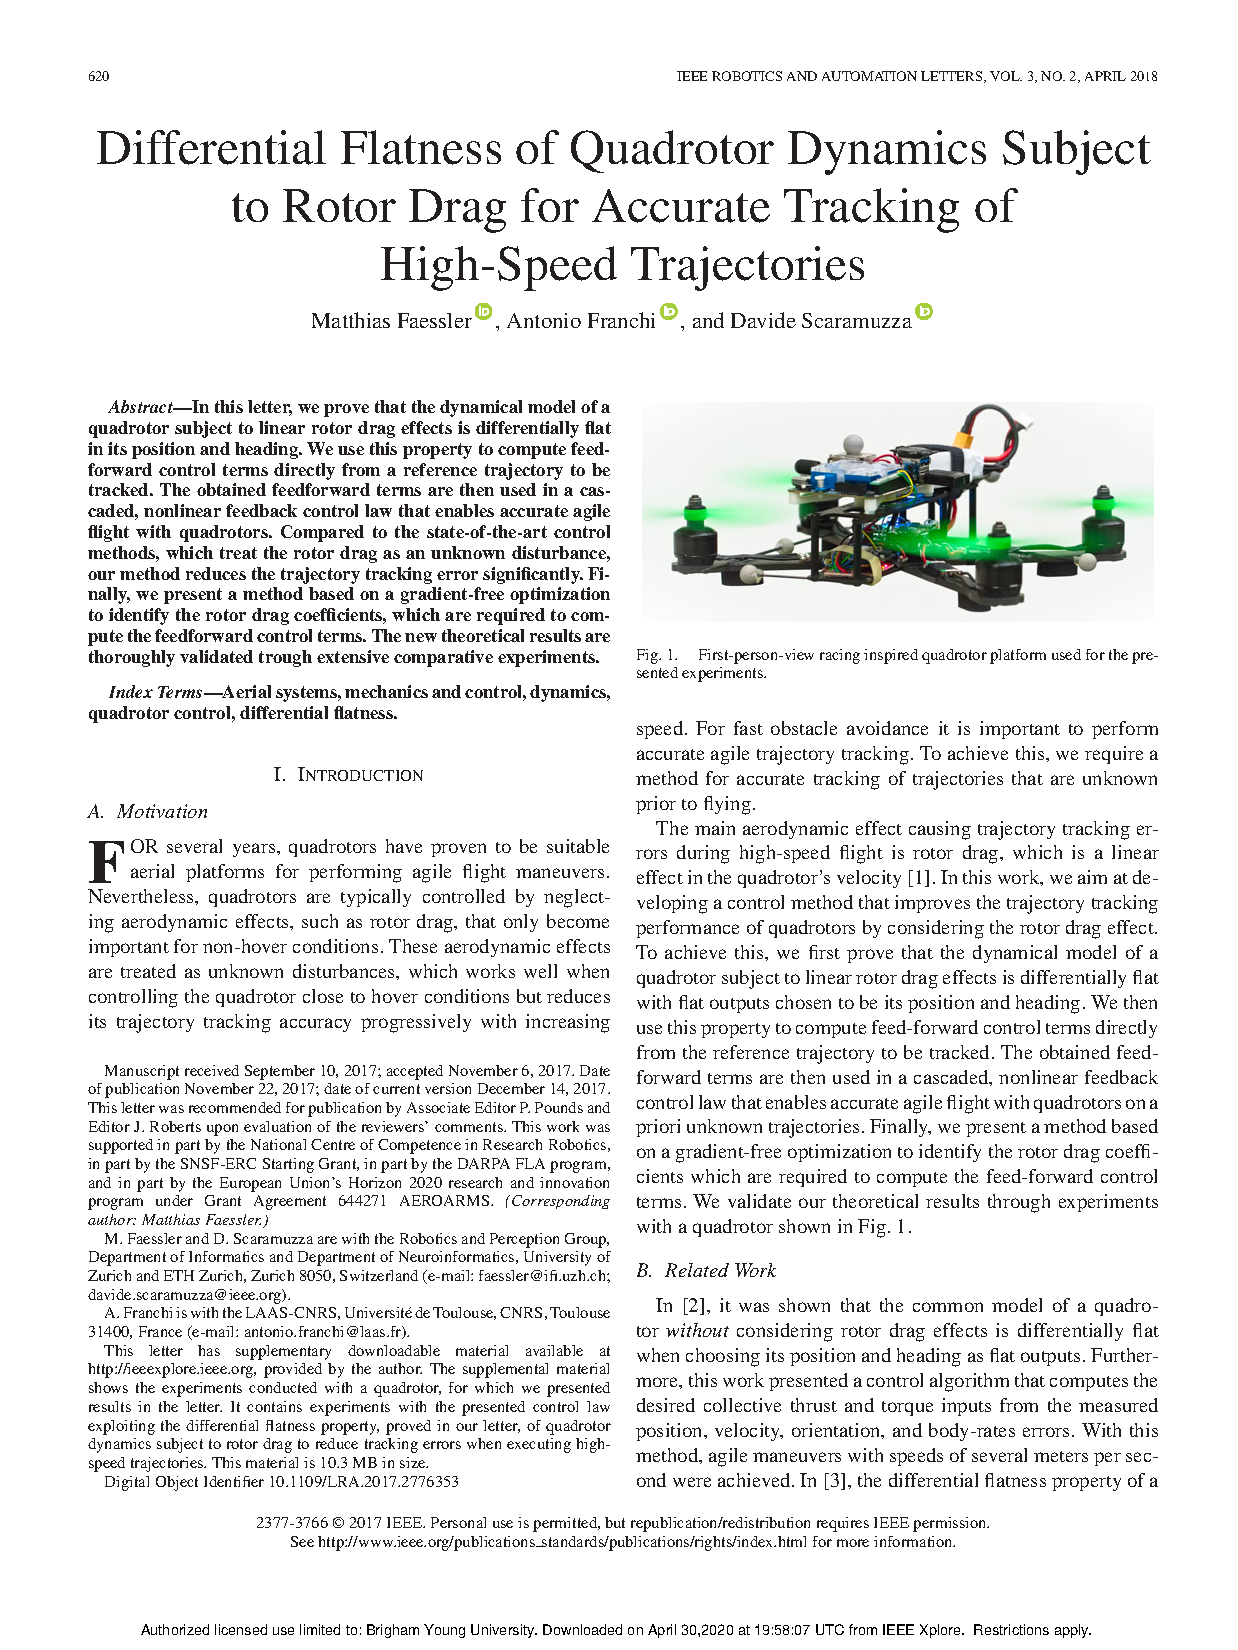
\includepdf[pages=-,scale=.8,pagecommand={}]{chap5_trajectory_planning/papers/FaesslerFranchiScaramuzza18.pdf}




%----------------------------------
\section{An Introduction to b-Spline}



%----------------------------------
\section{Minimum Snap Trajectory Generation}
Author:  Jacob Willis

Because multirotor dynamics are differentially flat, their motion can be completely parametrized by trajectories in position and heading.  It is common

it is desireable to be able to produce arbitrary 
trajectories for multirotors are frequently represented using piecewise polynomials.
Finding a trajectory is typically posed as an optimization problem where the objective is to minimize a certain derivative of the trajectory, given constraints such as waypoint locations and continuity of derivatives between segments.
In \cite{MellingerKumar11,RichterBryRoy16} this optimization is shown to be a constrained quadratic program and is solved using a conventional solver.
In this paper, I take a different approach, using dual approximation and least-squares to satisfy both segment endpoint constraints and to minimize the $k^\text{th}$ derivative along a single-dimensional, piecewise polynomial.

When generating a piecewise polynomial trajectory for a differentially flat system, we have three different priorities to consider.
\begin{enumerate}
	\item Knot point constraints. Position specified, and need to ensure that the spline is continuous up to the highest derivative taken in the flat map.
For a multirotor, this corresponds to the fourth derivative for the position splines, and to the second derivative for the yaw spline \cite{MellingerKumar11}.
We use a minimum norm method to acheive these constraints.
	\item Smoothness constraints. In (Mellinger \& Kumar, 2011)~\cite{MellingerKumar11}, the integral of the fourth derivative (snap) of the position splines 
and the second derivative of the yaw spline were minimized to produce multirotor trajectories. 
We acheive this constraint by operating in the nullspace of the knot point constraints.
This has a similar effect as minimizing the integral of the control effort.
	\item Vehicle dynamic constraints. It is possible to formulate the trajectory generation problem as a nonlinear optimization which computes the system states
and control inputs along the trajectory in order to meet constraints or optimize an objective. 
This, however, adds additional complexity to the trajectory generation, so we instead rely on the smoothness constraints described above, and time-scaling to
acheive dynamic constraints.
\end{enumerate}

\section{Notation}

\begin{figure*}
	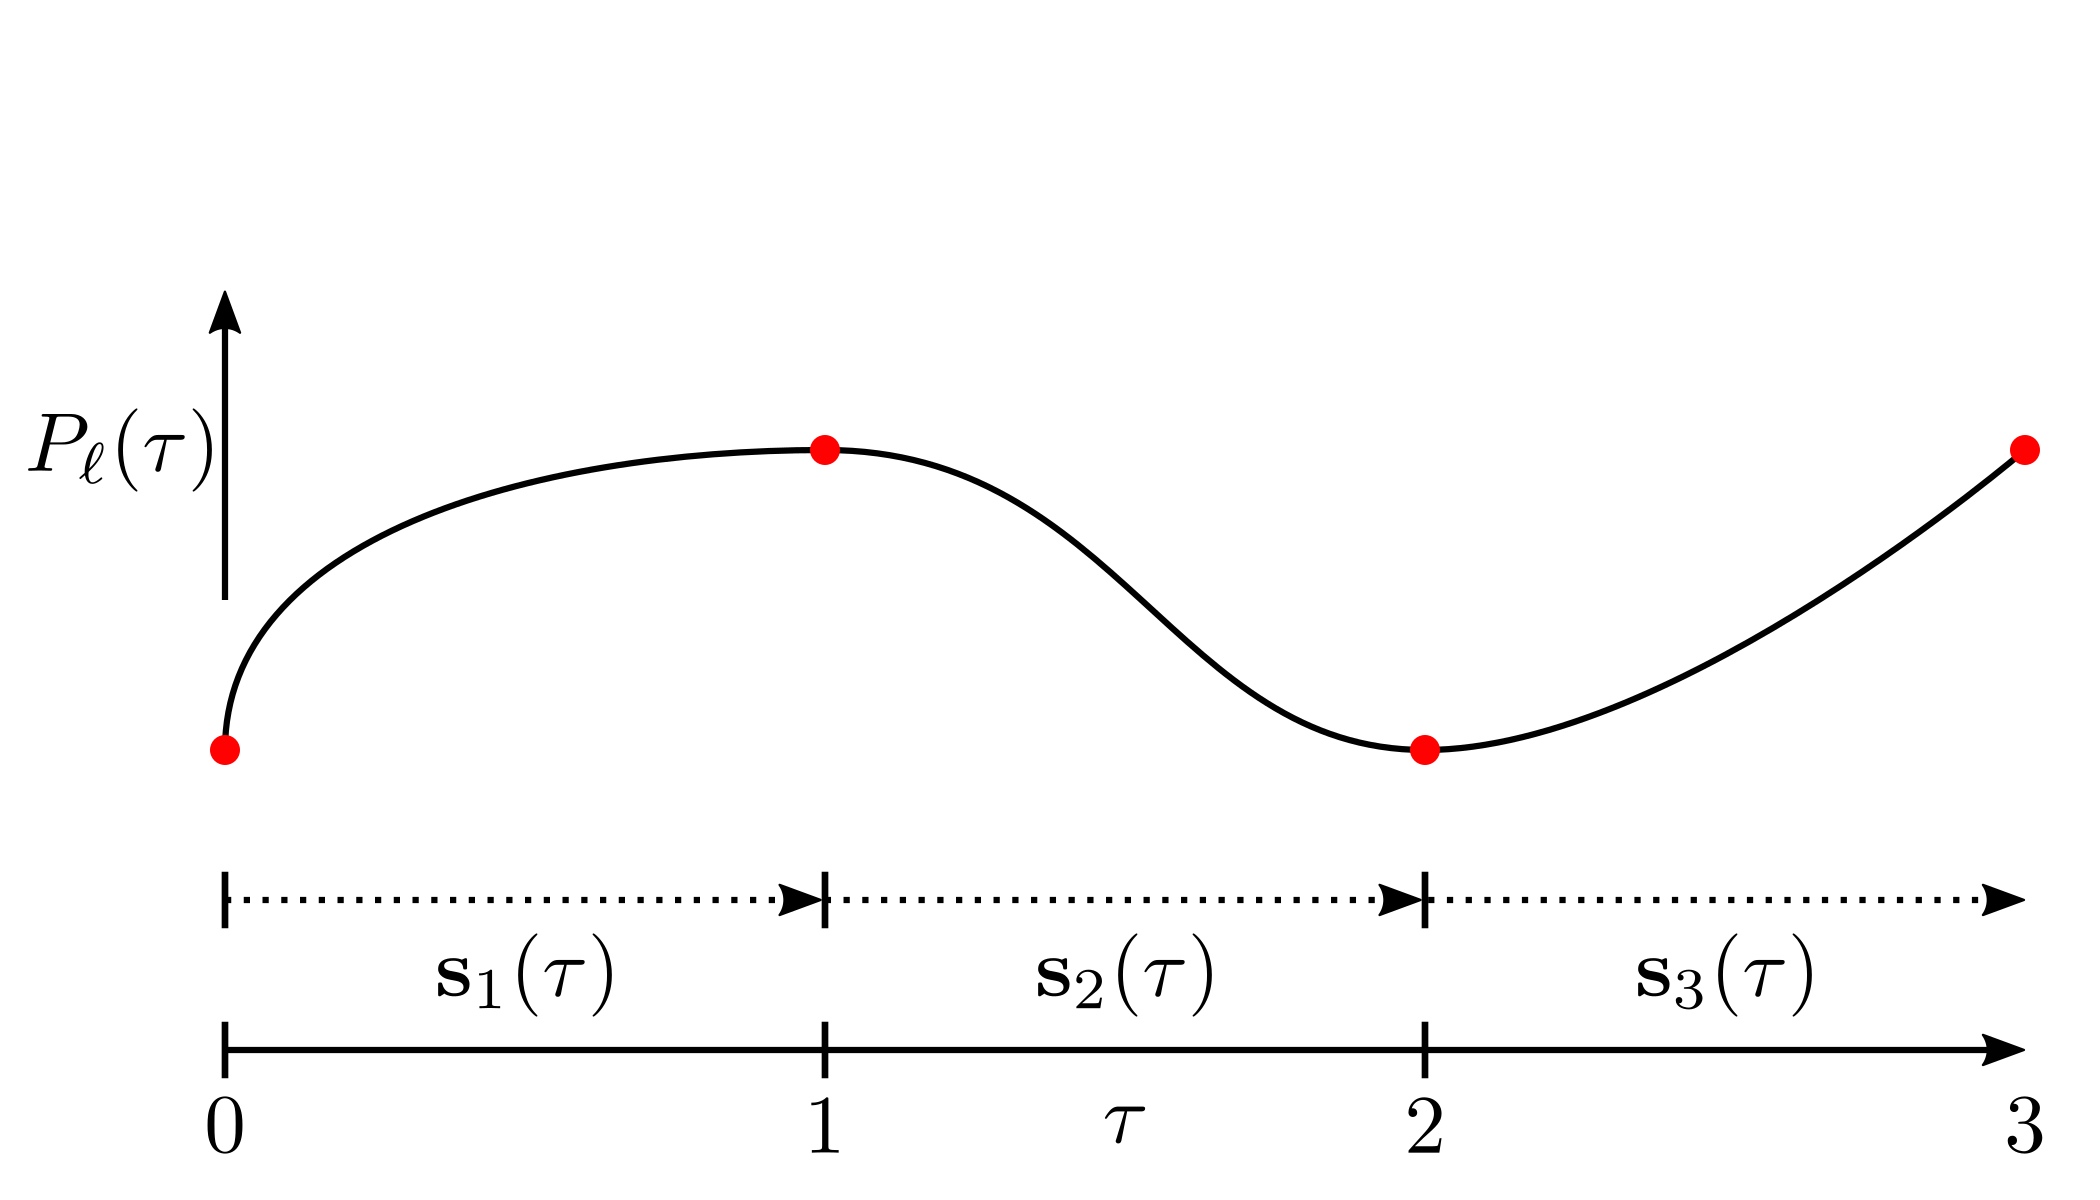
\includegraphics[width=\linewidth]{chap5_trajectory_planning/figures/trajectory_notation}
	\caption{Notation used for a single spline.}
	\label{fig:norm_accel_sol}
\end{figure*}

Let $P(\tau) = (P_1(\tau), P_2(\tau), \dots, P_r(\tau))$ be a set of $r$ splines, denoted $P_\ell(\tau)$, each of which is made up of $m$ segments, denoted $P_{\ell, i}(\tau)$,
where $\tau \in [0, m]$.
Each segment is parameterized by $s \in [0,1]$ and consists of the inner product of a vector of $n$ basis functions,
\begin{equation}
	\boldsymbol{\varphi}(s) = [\varphi_1(s), \varphi_2(s), \dots, \varphi_n(s)]^\top
\end{equation}
with $n$ coefficients $p_{\ell, i, j}$.
\marginnote{
	Choices for basis functions include the standard polynomials  
	$\boldsymbol{\varphi}(s) = [1, s, s^2, \dots, s^{n-1}]$, or the Legendre polynomials.
	Our implementation currently uses the standard polynomials.
}
We use a uniform spacing between segments, switching when $\tau\: \mathrm{mod}\: 1 = 0$.
To handle switching between segments, we define the basis vector for the $i^\text{th}$ segment as
\begin{equation}
	\mathbf{s}_i(\tau) = 
	\begin{cases} 
		\boldsymbol{\varphi}(s) & \text{for } i - 1 \leq \tau < i, \text{ with } s = \tau\: \mathrm{mod}\: i \\
		\mathbf{0}_n & \text{otherwise}
	\end{cases}
\end{equation}
where $\mathbf{0}_n$ is an $n \times 1$ vector of zeros.
Similarly, we define the $k^\text{th}$ derivative of 
$\mathbf{s}_i(\tau)$ with respect to $\tau$ as
 where
\begin{equation}
\mathbf{s}^{(k)}_i(\tau) \triangleq \frac{d^k \mathbf{s}(\tau)}{d\tau^k} = 
	\begin{cases} 
		\boldsymbol{\varphi}^{(k)} (s) & \text{for } i - 1 \leq \tau < i, \text{ with } s = \tau\: \mathrm{mod}\: i \\
		\mathbf{0}_n & \text{otherwise}
	\end{cases}
\end{equation}
where 
\begin{equation}
	\boldsymbol{\varphi}^{(k)} = [\varphi^{(k)}_1(s), \varphi^{(k)}_2(s), \dots, \varphi^{(k)}_n(s)]^\top
\end{equation}
and 
\begin{equation}
	\varphi_j^{(k)} \triangleq \frac{d^k\varphi}{ds^k}.
\end{equation}
Stacking these basis vectors, we get the $nm\times 1$ $\tau$-dependent vector
\begin{equation}
	\mathbf{S}(\tau) = 
	\begin{bmatrix} 
		\mathbf{s}_1(\tau)^\top, &
		\mathbf{s}_2(\tau)^\top, &
		\dots, &
		\mathbf{s}_m(\tau)^\top
	\end{bmatrix}^\top
\end{equation}
and
\begin{equation}
	\mathbf{S}^{(k)}(\tau) = 
	\begin{bmatrix} 
		\mathbf{s}_1^{(k)}(\tau)^\top, &
		\mathbf{s}_2^{(k)}(\tau)^\top, &
		\dots, &
		\mathbf{s}_m^{(k)}(\tau)^\top
	\end{bmatrix}^\top.
\end{equation}
Define the $n\times 1$ vector of segment coefficients for the $i^{\text{th}}$ segment of the $\ell^\text{th}$ spline to be
\begin{equation}
	\mathbf{p}_{\ell, i} = 
	\begin{bmatrix}
		p_{\ell, i, 1},& p_{\ell, i, 2},& \dots,& p_{\ell, i, n}
	\end{bmatrix}^\top,
\end{equation}
the $n m \times 1$ vector of all segment coefficients for the $\ell^\text{th}$ spline to be
\begin{equation}
	\mathbf{p}_{\ell} = 
	\begin{bmatrix}
	\mathbf{p}_{\ell, 1}^\top,& \mathbf{p}_{\ell, 2}^\top,& \dots,& \mathbf{p}_{\ell, n}^\top 
\end{bmatrix}^\top,
\end{equation}
and the $r \times n m$ matrix of segment coefficients for all splines to be 
\begin{equation}
	\mathbf{P} = 
	\begin{bmatrix} 
		\mathbf{p}_{1} &
		\mathbf{p}_{2} &
		\dots &
		\mathbf{p}_{r}
	\end{bmatrix}.
\end{equation}
Then, we can write 
\begin{equation}
	P_{\ell, i}(\tau) = \mathbf{p}_{\ell, i}^\top \mathbf{s}_i(\tau),
\end{equation}
\begin{equation}
	P_{\ell, i}^{(k)}(\tau) = \mathbf{p}_{\ell, i}^\top \mathbf{s}_i^{(k)}(\tau),
\end{equation}
\begin{equation}
	P_\ell(\tau) = \mathbf{p}_\ell^\top \mathbf{S}(\tau),
\end{equation}
\begin{equation}
	P_\ell^{(k)}(\tau) = \mathbf{p}_\ell^\top \mathbf{S}^{(k)}(\tau),
\end{equation}
\begin{equation}
	P(\tau) = \mathbf{P}^\top \mathbf{S}(\tau),
\end{equation}
and
\begin{equation}
	P^{(k)}(\tau) = \mathbf{P}^\top \mathbf{S}^{(k)}(\tau).
\end{equation}

\section{Satisfying knot point constraints}
\label{sec:knotpoint}
Knot point constraints ensure that the trajectory passes through desired waypoints, and that it is continuous at the desired knot points. 
Additionally, these constraints can be used to fix the derivatives of the trajectory at knot points.
This leads to two different types of constraints:
ensuring continuity of a derivative between two connecting segments, 
and fixing the value of a derivative at the endpoint of the segment. 
These can be written as inner products between $\mathbf{p}_\ell$ and $mn \times 1$ 
vectors consisting of zeros and one or more $\boldsymbol{\varphi}^{(k)}(s)$, evaluated at $0$ or $1$. 

First, we define the $mn \times 1$ vector with $\boldsymbol{\varphi}^{(k)} (s)$ in the $i^\text{th}$ position and zeros elsewhere as
\begin{equation}
	\Phi^{(k)}_{i} (s) = [\mathbf{0}_{n(i-1)}^\top, \boldsymbol{\varphi}^{(k)} (s)^\top, \mathbf{0}_{m(n-i)}^\top]^\top.
\end{equation}

\begin{theorem}
	Derivative continuity and knot point value constraints for a trajectory member $P_\ell(\tau)$ can be written as an inner product between 
	$\Phi^{(k)}_{i} (s)$ and $\mathbf{p}_\ell$.
\end{theorem}

\proof
	%Let $i = \floor{(\tau + 1)}$. Then, the values of $P_\ell(\tau)^{(k)}$ at its knot points are 
	The value of the starting knot points of segments in $P_\ell(\tau)$ are
	\begin{align}
		\mathbf{p}_\ell^\top \Phi^{(k)}_i (0) & \text{ for } i \in [1, n]
	\end{align}
	and the value of the ending knot points of segments in $P_\ell(\tau)$ are
	\begin{align}
		\mathbf{p}_\ell^\top \Phi^{(k)}_i (1) & \text{ for } i \in [1, n].
	\end{align}

	Thus, the $k^\text{th}$ derivative at the initial knot point of a segment $i$ can be set to a value $a$ by enforcing the constraint
	\begin{align}
		\mathbf{p}_\ell^\top \Phi^{(k)}_i (0) = a,
	\end{align}
	and the $k^\text{th}$ derivative at the final knot point of a segment $i$ can be set to a value $a$ by enforcing the constraint
	\begin{align}
		\mathbf{p}_\ell^\top \Phi^{(k)}_i (1) = a.
	\end{align}

	Continuity of the $k^\text{th}$ derivative between segments $i$ and $i+1$ can be ensured while allowing the value to vary by enforcing
	\begin{align}
		&\mathbf{p}_\ell^\top \Phi^{(k)}_i (1) = \mathbf{p}_\ell^\top \Phi^{(k)}_{i+1} (0)\\
		\Longleftrightarrow &\mathbf{p}_\ell^\top \Phi^{(k)}_i (1) - \mathbf{p}_\ell^\top \Phi^{(k)}_{i+1} (0) = 0\\
		\Longleftrightarrow &\mathbf{p}_\ell^\top (\Phi^{(k)}_i (1) - \Phi^{(k)}_{i+1} (0)) = 0
	\end{align}
\endproof

We let
\begin{equation}
\mathbf{a}_\ell^{(k_a)} = [a_{\ell,1}^{(k_a)}, a_{\ell,2}^{(k_a)}, \dots, a_{\ell,m+1}^{(k_a)}],
\end{equation}
denote the desired knot point locations ($k_a = 0$), or derivatives ($k_a > 0$) for the $\ell^\text{th}$ spline, 
where $\mathbf{a}_\ell^{(k_a)} \in \mathbb{R}^{c_{k_a}}$, with $c_{k_a} \leq m+1$.
It is possible to leave intermediate knot points free in their location or derivative, making $c_{k_a} < m+1$.
We use the convention that knot point 1 refers to the first knot point in the trajectory, 
and knot point $m+1$ refers to the final knot point.
The location or derivative constraints can be represented in matrix form with
\begin{equation}
	D^{(k_a)} \mathbf{p}_\ell = \mathbf{a}^{(k_a)}_\ell,
\end{equation}
defining the $m+1 \times mn$ matrix
\begin{equation}
	D^{(k_a)} \triangleq \begin{bmatrix}
		(\Phi^{(k_a)}_1(0))^\top \\
		(\Phi^{(k_a)}_2(0))^\top \\
		\vdots\\
		(\Phi^{(k_a)}_m(1))^\top 
	\end{bmatrix}.
\end{equation}
With $k_{a,\text{max}}$ being the highest derivative at which the value or derivatives of a knot point
is fixed, we let
\begin{equation}
	\bar{\mathbf{a}}_\ell = \begin{bmatrix}
		\mathbf{a}^{(0)}_\ell, \\
		\mathbf{a}^{(1)}_\ell, \\
		\vdots \\
		\mathbf{a}^{(k_{a,\text{max}})}_\ell, \\
	\end{bmatrix}
\end{equation}
whose length we denote to be $c_a$.


Similarly, the intermediate knot point continuity constraints for the $k_\ell^\text{th}$ derivative can be represented in matrix form as
\begin{equation}
	D_c^{(k_\ell)} \mathbf{p}_\ell = \mathbf{0}_{m-1}
\end{equation}
with the $m-1 \times mn$ matrix
\begin{equation}
	D_c^{(k_\ell)} \triangleq \begin{bmatrix}
		(\Phi^{(k_\ell)}_1 (1) - \Phi^{(k_\ell)}_{2} (0))^\top \\
		(\Phi^{(k_\ell)}_2 (1) - \Phi^{(k_\ell)}_{3} (0))^\top \\
		\vdots \\
		(\Phi^{(k_\ell)}_{m-1} (1) - \Phi^{(k_\ell)}_{m} (0))^\top 
	\end{bmatrix}.
\end{equation}
If $k_{\ell,\text{max}}$ is the highest order of derivative for which we wish to enforce continuity at the knot points,
there will be $(m-1) k_{\ell,\text{max}}$ continuity constraints. 
We then define
\begin{equation}
	\mathbf{a}_\ell = \begin{bmatrix} \bar{\mathbf{a}}_\ell \\ \mathbf{0}_{(m-1)k_{\ell,\text{max}}} \end{bmatrix}
\end{equation}
to be a vector of length $c = c_a + (m-1)k_{\ell,\text{max}}$, and the $c \times r$ matrix
\begin{equation}
\mathbf{A} = \begin{bmatrix} \mathbf{a}_1 & \mathbf{a}_2 & \dots & \mathbf{a}_r \end{bmatrix}
\end{equation}.  
We can then formulate the knot point constraints for all of the splines in matrix form as
\begin{equation}
	\label{eq:knot_con}
	\mathbf{D} \mathbf{P} = \mathbf{A}
\end{equation}
where
\begin{equation}
	\mathbf{D} = 
	\begin{bmatrix}
		D^{(0)}\\
		\vdots \\
		D^{(k_{a,\text{max}})}\\
		D_c^{(0)} \\
		\vdots\\
		D_c^{(k_{\ell, \text{max}})}
	\end{bmatrix} \in \mathbb{R}^{c \times mn}.
\end{equation}

By choosing $n$ such that $mn > c$, $\mathbf{D}$ will be wide, and Eq.~\ref{eq:knot_con} will be an under determined system with $mn - c$ remaining degrees of freedom.
We assume that $\rank{(\mathbf{D})} = c$; if $\rank{(\mathbf{D})} < c$, there are linearly dependent constraints that can be removed from $\mathbf{D}$.

As shown in \cite{MoonStirling00}, the singular value decomposition (SVD)
can be used to find the solution to Eq.~\ref{eq:knot_con} of minimum norm.
Generally, the SVD of an $n \times m$ matrix $\mathbf{X}$ with rank $r$ is 
\begin{equation}
	\mathbf{X} = U \Sigma V^\top = 
	\begin{bmatrix} U_1 & U_2 \end{bmatrix} 
	\begin{bmatrix} \Sigma_1 & \\ & \Sigma_2 \end{bmatrix} 
	\begin{bmatrix} V_1^\top \\ V_2^\top \end{bmatrix},
	\label{eq:D_svd}
\end{equation}
where $U \in \mathbb{R}^{n \times n}$, $V \in \mathbb{R}^{m \times m}$, and $\Sigma \in \mathbb{R}^{n \times m}$, with
$U_1 \in \mathbb{R}^{n \times r}$, $U_2 \in \mathbb{R}^{n \times (n-r)}$,
$\Sigma_1 \in \mathbb{R}^{r \times r}$, $\Sigma_2 \in \mathbb{R}^{(n-r) \times (m-r)}$,
$V_1 \in \mathbb{R}^{m \times r}$, and $V_2 \in \mathbb{R}^{m \times (m-r)}$.
Noting that since $\rank{(\mathbf{D})} = c$, 
\begin{equation}
	\mathbf{D} = U \Sigma V^\top = 
	U 
	\begin{bmatrix} \Sigma_1 & \Sigma_2 \end{bmatrix} 
	\begin{bmatrix} V_1^\top \\ V_2^\top \end{bmatrix},
	\label{eq:D_svd}
\end{equation}
where $U \in \mathbb{R}^{c \times c}$, $V \in \mathbb{R}^{mn \times mn}$, and $\Sigma \in \mathbb{R}^{c \times mn}$, with
$\Sigma_1 \in \mathbb{R}^{c \times c}$, $\Sigma_2 \in \mathbb{R}^{c \times mn-c}$,
$V_1 \in \mathbb{R}^{mn \times c}$, and $V_2 \in \mathbb{R}^{mn \times (mn-c)}$.
Because it is not of full column rank, $\mathbf{D}$ has a nontrivial nullspace which is spanned by the columns of $V_2$.
Solutions to Eq.~\ref{eq:knot_con} are then
\begin{equation}
	\label{eq:P_svd_sol}
	\mathbf{P} = \bar{\mathbf{P}} + V_2 \mathbf{B} = V_1 \Sigma_1^{-1} U^\top \mathbf{A} + V_2 \mathbf{B}
\end{equation}
where $\bar{\mathbf{P}}$ is the minimum norm solution to Eq.~\ref{eq:knot_con}, and $\mathbf{B} \in \mathbb{R}^{(mn-c) \times r}$.

Thus, a polynomial trajectory satisfying the constraints given by $\mathbf{D}$ and $\mathbf{A}$ is
\begin{equation}
	P(\tau) = \mathbf{P}^\top \mathbf{S}(\tau).
\end{equation}

\section{Minimizing the $k^\mathrm{th}$ derivative}
Beyond satisfying knot point constraints, it is common \cite{RichterBryRoy16,MellingerKumar11} 
to minimize the integral of some derivative $k_r$ of $P(\tau)$ over the length of the trajectory,
\begin{equation}
	\label{eq:min_derivative}
	\begin{aligned}
	&\min_{\mathbf{P}} \int_{0}^m \|P^{(k_r)}(\tau)\|^2 d\tau \\
	&\text{subject to } \: \mathbf{D}\mathbf{P} = \mathbf{A}. 
	\end{aligned}
\end{equation}
The choice of $k_r$ is typically chosen to be one higher than the highest derivative needed to perform control. 
For a quadroter, snap ($k_r = 4$) is often minimized~\cite{MellingerKumar11}.


We now consider the solution to this optimization.
\begin{theorem}
	With 
	\begin{equation}
		\mathbf{W} \triangleq \int_0^m \mathbf{S}^{(k_r)}(\tau) (\mathbf{S}^{(k_r)} (\tau))^\top d\tau
	\end{equation}
	the optimization in Eq.~\ref{eq:min_derivative} has the analytic solution
	\begin{equation}
		\mathbf{P}^\star = \mathbf{H} \mathbf{A}
	\end{equation}
	where
	\begin{equation}
		 \mathbf{H}  = (\mathbf{I}_{mn \times mn} - V_2(V_2^\top \mathbf{W} V_2)^{-1} V_2^\top \mathbf{W})V_1 \Sigma^{-1} U^\top.
	\end{equation}
\end{theorem}
\proof
	As indicated by Eq.~\ref{eq:P_svd_sol}, there are infinitely many trajectories satisfying Eq.~\ref{eq:knot_con}.
	By modifying $\mathbf{B}$, the remaining degrees of freedom in Eq.~\ref{eq:knot_con} can be utilized to achieve a secondary objective. 
	To this end, we reformulate Eq.~\ref{eq:min_derivative} to be an unconstrained optimization over $\mathbf{B}$:
	\begin{equation}
		\label{eq:min_derivative_uncon}
		\begin{aligned}
		&\min_{\mathbf{B}} \int_{0}^m \|P^{(k_r)}(\tau)\|^2 d\tau. 
		\end{aligned}
	\end{equation}
	We then have
	\begin{align}
		&\min_{\mathbf{B}} \int_{0}^m \|P^{(k_r)}(\tau)\|^2 d\tau \\
		&= \min_{\mathbf{B}} \int_{0}^m (\mathbf{P}^\top \mathbf{S}^{(k_r)}(\tau))^\top \mathbf{P}^\top \mathbf{S}^{(k_r)}(\tau)  d\tau \\
		&= \min_{\mathbf{B}} \int_{0}^m (\mathbf{P}^\top \mathbf{S}^{(k_r)}(\tau))^\top \mathbf{P}^\top \mathbf{S}^{(k_r)}(\tau)  d\tau \\
		&= \min_{\mathbf{B}} \int_{0}^m  (\mathbf{S}^{(k_r)}(\tau)^\top \mathbf{P} \mathbf{P}^\top \mathbf{S}^{(k_r)}(\tau)  d\tau \\
		&= \min_{\mathbf{B}} \mathrm{tr} \left\{ \int_{0}^m  (\mathbf{S}^{(k_r)}(\tau)^\top \mathbf{P} \mathbf{P}^\top \mathbf{S}^{(k_r)}(\tau)  d\tau \right\} \\
		&= \min_{\mathbf{B}} \mathrm{tr} \left\{ \int_{0}^m \mathbf{P}^\top \mathbf{S}^{(k_r)}(\tau)  (\mathbf{S}^{(k_r)}(\tau)^\top \mathbf{P}  d\tau \right\} \\
		&= \min_{\mathbf{B}} \mathrm{tr} \left\{ \mathbf{P}^\top \mathbf{W} \mathbf{P}  \right\}
	\end{align}
	where
	\begin{equation}
		\mathbf{W} \triangleq \int_0^m \mathbf{S}^{(k_r)}(\tau) (\mathbf{S}^{(k_r)} (\tau))^\top d\tau. 
	\end{equation}
	Noting that $\mathbf{W}$ is independent of $\mathbf{B}$, it can be seen that this optimization takes a quadratic form.

	Substituting $\mathbf{P} = \bar{\mathbf{P}} + V_2 \mathbf{B}$, we have
	\begin{align}
		&\min_{\mathbf{B}} \mathrm{tr} \left\{ \mathbf{P}^\top \mathbf{W} \mathbf{P}  \right\} \\
		&= \min_{\mathbf{B}} \mathrm{tr} \left\{ (\bar{\mathbf{P}} + V_2\mathbf{B})^\top \mathbf{W} (\bar{\mathbf{P}} + V_2\mathbf{B})  \right\}\\
		&= \min_{\mathbf{B}} \mathrm{tr} \left\{ (\bar{\mathbf{P}} + V_2\mathbf{B})^\top \mathbf{W} (\bar{\mathbf{P}} + V_2\mathbf{B})  \right\}\\
		&= \min_{\mathbf{B}} \mathrm{tr} \left\{ (\bar{\mathbf{P}})^\top \mathbf{W}\bar{\mathbf{P}} + \mathbf{B}^\top V_2^\top \mathbf{W} V_2 \mathbf{B}
		+ 2 \mathbf{B}_\ell^\top V_2^\top \mathbf{W}\bar{\mathbf{P}} \right\}
	\end{align}
	which is quadratic in $\mathbf{B}$.
	Taking the gradient, $\frac{\partial}{\partial \mathbf{B}_\ell}$ we have
	\begin{align}
		&2 V_2^\top \mathbf{W} V_2 \mathbf{B} + 2 V_2^\top \mathbf{W}\bar{\mathbf{P}}.
	\end{align}
	Setting to zero, we find that
	\begin{align}
		\mathbf{B}^\star = - (V_2^\top \mathbf{W} V_2)^{-1} V_2^\top \mathbf{W} \bar{\mathbf{P}}.
	\end{align}
	Now,
	\begin{align}
		\mathbf{P}^\star &= \bar{\mathbf{P}} + V_2 \mathbf{B}^\star \\
		&= (\mathbf{I}_{mn \times mn} - V_2  (V_2^\top \mathbf{W} V_2)^{-1} V_2^\top \mathbf{W}) \bar{\mathbf{P}}\\
		&= (\mathbf{I}_{mn \times mn} - V_2  (V_2^\top \mathbf{W} V_2)^{-1} V_2^\top \mathbf{W}) V_1 \Sigma^{-1} U^\top A
	\end{align}

\endproof

We now investigate the structure of $\mathbf{W}$ in more detail.
Letting $\mathbf{s}_i^{(k_r)}(\tau) = \mathbf{s}_i$ we have
\begin{align}
	\mathbf{W} &\triangleq \int_0^m \mathbf{S}^{(k_r)}(\tau) (\mathbf{S}^{(k_r)} (\tau))^\top d\tau. \\
	&= \int_0^m 
	\begin{bmatrix}
		\mathbf{s}_1 \\		
		\mathbf{s}_2 \\		
		\vdots \\
		\mathbf{s}_m
	\end{bmatrix}
	\begin{bmatrix}
		\mathbf{s}_1 &
		\mathbf{s}_2 &
		\dots &
		\mathbf{s}_m 
	\end{bmatrix} d\tau \\
	&= \int_0^m 
	\begin{bmatrix}
		\mathbf{s}_1 \mathbf{s}_1^\top & \mathbf{s}_1 \mathbf{s}_2^\top & \dots & \mathbf{s}_1 \mathbf{s}_m^\top\\		
		\mathbf{s}_2 \mathbf{s}_1^\top & \mathbf{s}_2 \mathbf{s}_2^\top & \dots & \mathbf{s}_2 \mathbf{s}_m^\top\\		
		\vdots & \vdots & \ddots & \vdots \\
		\mathbf{s}_m \mathbf{s}_1^\top & \mathbf{s}_m \mathbf{s}_2^\top & \dots & \mathbf{s}_m \mathbf{s}_m^\top\\		
	\end{bmatrix} d\tau. 
	\label{eq:int_s_grammian_full}
\end{align}
Since $\mathbf{s}^{(k_r)}_i(\tau) = \mathbf{0}_n$ for $\tau \not\in [i, i+1]$, and 
$\mathbf{s}^{(k_r)}_i(\tau) = \boldsymbol{\varphi}^{(k_r)}(s)$ for $\tau \in [i, i+1]$ with $s = \tau\:\text{mod}\:i$,
the cross terms $\mathbf{s}_i \mathbf{s}_j^\top$ for $i \neq j$ in Eq.~\ref{eq:int_s_grammian_full} evaluate to zero.
This makes $\mathbf{W}$ block diagonal.
Additionally, each of the diagonal terms is identical, giving us $\mathbf{W} = \mathrm{diag}(W, W, \dots, W)$, where
${W} \in \mathbb{R}^{n \times n}$ is the integral of a diagonal term of Eq.~\ref{eq:int_s_grammian_full}:
\begin{align}
	&{W} \triangleq \int_0^m \mathbf{s}^{(k_r)}_i(\tau) (\mathbf{s}^{(k_r)}_i(\tau))^\top d\tau \\
	=& \int_0^1 \boldsymbol{\varphi}^{(k_r)}(s) (\boldsymbol{\varphi}^{(k_r)}(s))^\top ds \\
	=& \int_0^1 
	\begin{bmatrix}
		(\varphi_1^{(k_r)}(s))^2 & \varphi_1^{(k_r)}(s) \varphi_2^{(k_r)}(s) & \dots & \varphi_1^{(k_r)}(s) \varphi_n^{(k_r)}(s)\\		
		\varphi_2^{(k_r)}(s) \varphi_1^{(k_r)}(s) & (\varphi_2^{(k_r)}(s))^2 & \dots & \varphi_2^{(k_r)}(s) \varphi_n^{(k_r)}(s)\\		
		\vdots & \vdots & \ddots & \vdots \\
		\varphi_n^{(k_r)}(s) \varphi_1^{(k_r)}(s) & \varphi_n^{(k_r)}(s) \varphi_2^{(k_r)}(s) & \dots & (\varphi_n^{(k_r)}(s))^2\\		
	\end{bmatrix} ds. 
\end{align}
It can be seen that $W$ is symmetric, and positive semi-definite.
If the basis members $\varphi_j$ are orthogonal, then ${W}$ is diagonal. 
If $k_r > 0$ (which, in general, will be true), then $\varphi_j^{(k_r)} = 0$ for $j < k_r$, making ${W}$ singular.
\jbwcomment{I have found that $V_2^\top \mathbf{W} V_2$ is full rank, so I think there is some more investigation we can do here.}

%\jbwcomment{ This is a really interesting result (assuming my math is correct). What we really care about is finding $\mathbf{r}_\ell$, since that is what will actually be applied to the trajectory. In general, $\mathbf{W}$ will be singular. Additionally, $V_2^T\mathbf{W}$ will be $(mn - c) \times mn$ (tall), so solving here for $\mathbf{r}_\ell$ will be approximate - or will we just get $\mathbf{r} = 0$?. In that case, $\mathbf{W}$ is irrelevant, and we only need to find $\mathbf{b}_\ell$ such that $\|V_2 \mathbf{b}_\ell + \mathbf{p}^\star_\ell\|$ is minimized, ie $\mathbf{b}_\ell = -V_2^\dagger \mathbf{p}$. That's a pretty cool result if that is the case, as it would also imply that it is true for minimizing any derivative - including the zeroth, so the minimum snap trajectory would also be minimum accel, velocity, and length.}



%--------------------------------------------------------------------------------
%--------------------------------------------------------------------------------
%--------------------------------------------------------------------------------

\section{Ensuring dynamic feasibility using time scaling}
The dynamics of a differentially flat system can be satisfied by planning in the flat output space. 
However, these dynamic models typically neglect system limitations such as actuator saturation. 
It is possible to include system limits in the trajectory optimization. 
These limits typically yield non-convex constraints, requiring a nonlinear optimizer to solve.
Instead of directly constraining the system, we use time scaling to ensure the constraints are satisfied.

Let 
\begin{equation}
\tau = \alpha t, 
\end{equation}
where $t$ is dimensional time. 
We then define the trajectory $P(t) = P(\tau(t))$, and the system dynamic constraints to be a nonlinear function of the trajectory and its derivatives:
\begin{equation}
	C(P(t), P^{(1)}(t), \dots, P^{(k)}(t)).
\end{equation}

\begin{theorem}
	The derivatives of $P(t)$ with respect to $t$ can be written as
	\begin{equation}
		\frac{d^{k}} {dt^k}  = \alpha^k \frac{d^k P}{d\tau^k}
	\end{equation}
\end{theorem}
\proof
Should probably be by induction\dots

With $P(t) = P(\alpha t)$, and noting that $\frac{d\tau}{dt} = \alpha$, by the chain rule we have
\begin{align}
\frac{dP}{dt} &= \frac{dP}{d\tau}\frac{d\tau}{dt} = \alpha \frac{dP}{d\tau} \\
\frac{d^2P}{dt^2} &= \frac{d}{dt} \left( \alpha \frac{dP}{d\tau} \right) = \alpha \frac{d^2P}{d\tau^2}\frac{d\tau}{dt} = \alpha^2 \frac{d^2P}{d\tau^2}  \\
\frac{d^3P}{dt^3} &= \frac{d}{dt} \left( \alpha^2 \frac{d^2P}{d\tau^2} \right) = \alpha^2 \frac{d^3P}{d\tau^3}\frac{d\tau}{dt} = \alpha^3 \frac{d^3P}{d\tau^3} \\
&\vdots
\end{align}
\endproof

%%% end Jacob Willis stuff




\rwbcomment{Replace this section with Jacob Willis' stuff.}

If a system is differentially flat with flat output $z$, then the open-loop path planning problem presumably becomes much easier.  If there are no constraints on the state and input variables, then planning becomes trivial.  If there are constraints, then the planning problem can be reduced to a constrained optimization problem.

%+++++++++++++++++++++++++++++++++++++++++++++++++
\subsection{Path planning without constraints}
Suppose that the objective is to plan a path from a start position $p_s$ and a start velocity $p_s^{'}$, to an end position $p_e$ and an end velocity $p_e^{'}$.  Instead of parameterizing the path by time $t$, we will use the path parameter $\sigma$.  This will allow us to later specify the velocity by creating dynamics for $\sigma(t)$.  Let  $p:[0,T]\to\re^3$ denote the path.  The path will be given by the finite series expansion
\begin{align*}
p(\sigma) &= \begin{pmatrix} \sum_{j=1}^N c_{1j} \phi_j(\sigma) \\  \sum_{j=1}^N c_{2j} \phi_j(\sigma) \\  \sum_{j=1}^N c_{3j} \phi_j(\sigma) \end{pmatrix} \\
&= C\phi(t),
\end{align*}
where 
\[
C = \begin{pmatrix} c_{11} & c_{12} & \dots & c_{1N} \\ c_{21} & c_{22} & \dots & c_{2N} \\c_{31} & c_{32} & \dots & c_{3N} \end{pmatrix},
\]
and
\[
\phi(\sigma) = \begin{pmatrix} \phi_1(\sigma) & \phi_2(\sigma) & \dots & \phi_N(\sigma) \end{pmatrix}^{\top},
\]
and where $\{\phi_j(\sigma)\}$ are the basis functions.  For example, for a polynomial basis we have $\phi_j(\sigma)=\sigma^j/j!$. We also define the derivative of the basis function as
\[
\phi_j^{'}(\sigma)\defeq\frac{d\phi_j}{d\sigma}(\sigma),
\]
and 
\[
\phi^{'}(\sigma) = \begin{pmatrix} \phi_1^{'}(\sigma) & \phi_2^{'}(\sigma) & \dots & \phi_N^{'}(\sigma) \end{pmatrix}^{\top}.
\]

For the path the start at $p_s$ we must have
\[
p_s = p(0)= C\phi(0).
\]
For the start velocity to be $p_s^{'}$ we must have
\[
p_s^{'} = p^{'}(0) = C\phi^{'}(0).
\]
For the path to end at $p_e$ we need
\[
p_e = p(T)= C\phi(T),
\]
and for the end velocity to be $p_e^{'}$ we require that
\[
p_e^{'} = p^{'}(T) = C\phi^{'}(T).
\]
Since $\sigma$ is a path parameterization, without loss of generality we will let $\sigma$ at the endpoint equal to $T=1$.

Defining 
\begin{align*}
P &\defeq \begin{pmatrix} p_s & p_s^{'} & p_e & p_e^{'} \end{pmatrix} \\
\Phi &\defeq \begin{pmatrix} \phi(0) & \phi^{'}(0) & \phi(1) & \phi^{'}(1) \end{pmatrix}
\end{align*}
we have that the coefficients $C$ must satisfy
\begin{equation}\label{eq:flat-coefficient-equation}
C\Phi = P.  
\end{equation}

Let the singular value decomposition for $\Phi$ be given by $\Phi = \begin{bmatrix}U_1 & U_2\end{bmatrix}\begin{bmatrix}\Sigma \\ \mathbf{0} \end{bmatrix}V^\top = U_1\Sigma V^\top$, where 
$U_1\in\mathbb{R}^{N\times 4}$, $U_2\in\mathbb{R}^{N\times (N-4)}$, $\Sigma\in\mathbb{R}^{4\times 4}$, and $V\in\mathbb{R}^{4\times 4}$, and where $U_1^\top U_1 = I$, $U_2^\top U_2=I$, $U_1^\top U_2 = 0$, and $U_2^\top U_1=0$.  Letting
\[
C = PV\Sigma^{-1}U_1^\top + BU_2^\top,
\]
where $B\in\mathbb{R}^{3\times (N-4)}$ can be arbitrarily selected, then 
\begin{align*}
C\Phi &= (PV\Sigma^{-1}U_1^\top + BU_2^\top)U_1\Sigma V^\top \\
      &= PV\Sigma^{-1}\Sigma V^\top = P V V^\top \\
      &= P.
\end{align*}

The first term $PV\Sigma^{-1}U_1^\top$ is the minimum norm solution to the path planning problem.  The second term $BU_2^\top$ represents a parameterization of the corresponding null space.  Given additional constraints, the matrix $B$ can be selected to satisfy those constraints.


%+++++++++++++++++++++++++++++++++++++++++++++++++
\subsection{Time Parameterization}
The path can be time parameterized by letting $\sigma$ be a function of time, where we require that $\frac{d\sigma}{dt}>0$ to ensure a forward looking parameterization of the path.  If we desire a fixed speed $v^d$ along the path, then 
\begin{align*}
v^d &= \norm{\frac{d}{dt}p(\sigma(t))} \\
&= \norm{\frac{\partial p}{\partial\sigma}\frac{d\sigma}{dt}} \\
&= \norm{C\phi'(\sigma(t))}\frac{d\sigma}{dt}.
\end{align*}
Therefore, $\sigma$ should satisfy the differential equation
\[
\frac{d\sigma}{dt} = \frac{v^d}{\norm{C\phi'(\sigma(t))}}.
\]

The path length is dependent only on the parameter $\sigma$ and is given by
\begin{align*}
L &= \int_0^1 \norm{p'(\sigma)}d\sigma \\
  &= \int_0^1 \norm{C\phi'(\sigma)}d\sigma.
\end{align*}
Sampling $\sigma$ at a finite number of values $0\leq\sigma_1\leq\sigma_2\leq\dots\leq\sigma_N\leq 1$, the path length is approximated as
\[
L \approx \sum_{i=2}^N \norm{C\phi'(\sigma_i)}\abs{\sigma_i-\sigma_{i-1}}.
\]

    


%+++++++++++++++++++++++++++++++++++++++++++++++++
\subsection{Path planning with constraints}


If $N>4$, then $\Phi^\top$ has a non-trivial null space that can be exploited to satisfy additional constraints.  As an example, we may want to minimize the curvature of the path.  

The curvature of $p(\sigma)$ is defined by the formula
\[
\kappa(\sigma) = \frac{p^{'}(\sigma)\times p^{''}(\sigma)}{\norm{p^{'}(\sigma)}^3}.
\]
Since the path $p(\sigma)$ is also a function of the null space parametrization $B$, we write $p(\sigma, B)$, and so
\[
\kappa(\sigma, B) = \frac{p^{'}(\sigma, B)\times p^{''}(\sigma, B)}{\norm{p^{'}(\sigma, B)}^3}.
\]
To solve the path planning problem subject to a minimum curvature constraint, we need to solve the following optimization problem:
\[
B^\ast = \arg\min_{B\in\mathbb{R}^{3\times(N-4)}} \left\{ \max_{\sigma\in[0,1]}\kappa(\sigma, B)\right\}.
\]
To make the problem tractable, we can sample $\sigma$ at a finite number of values $0\leq\sigma_1\leq\sigma_2\leq\dots\leq\sigma_N\leq 1$, and solve
\[
B^\ast = \arg\min_{B\in\mathbb{R}^{3\times(N-4)}} \left\{ \max_{i=1,\dots,N}\kappa(\sigma_i, B)\right\}.
\]

\subsection{Minimum Snap Trajectory Generation and Control for Quadrotors, ICRA, 2011}
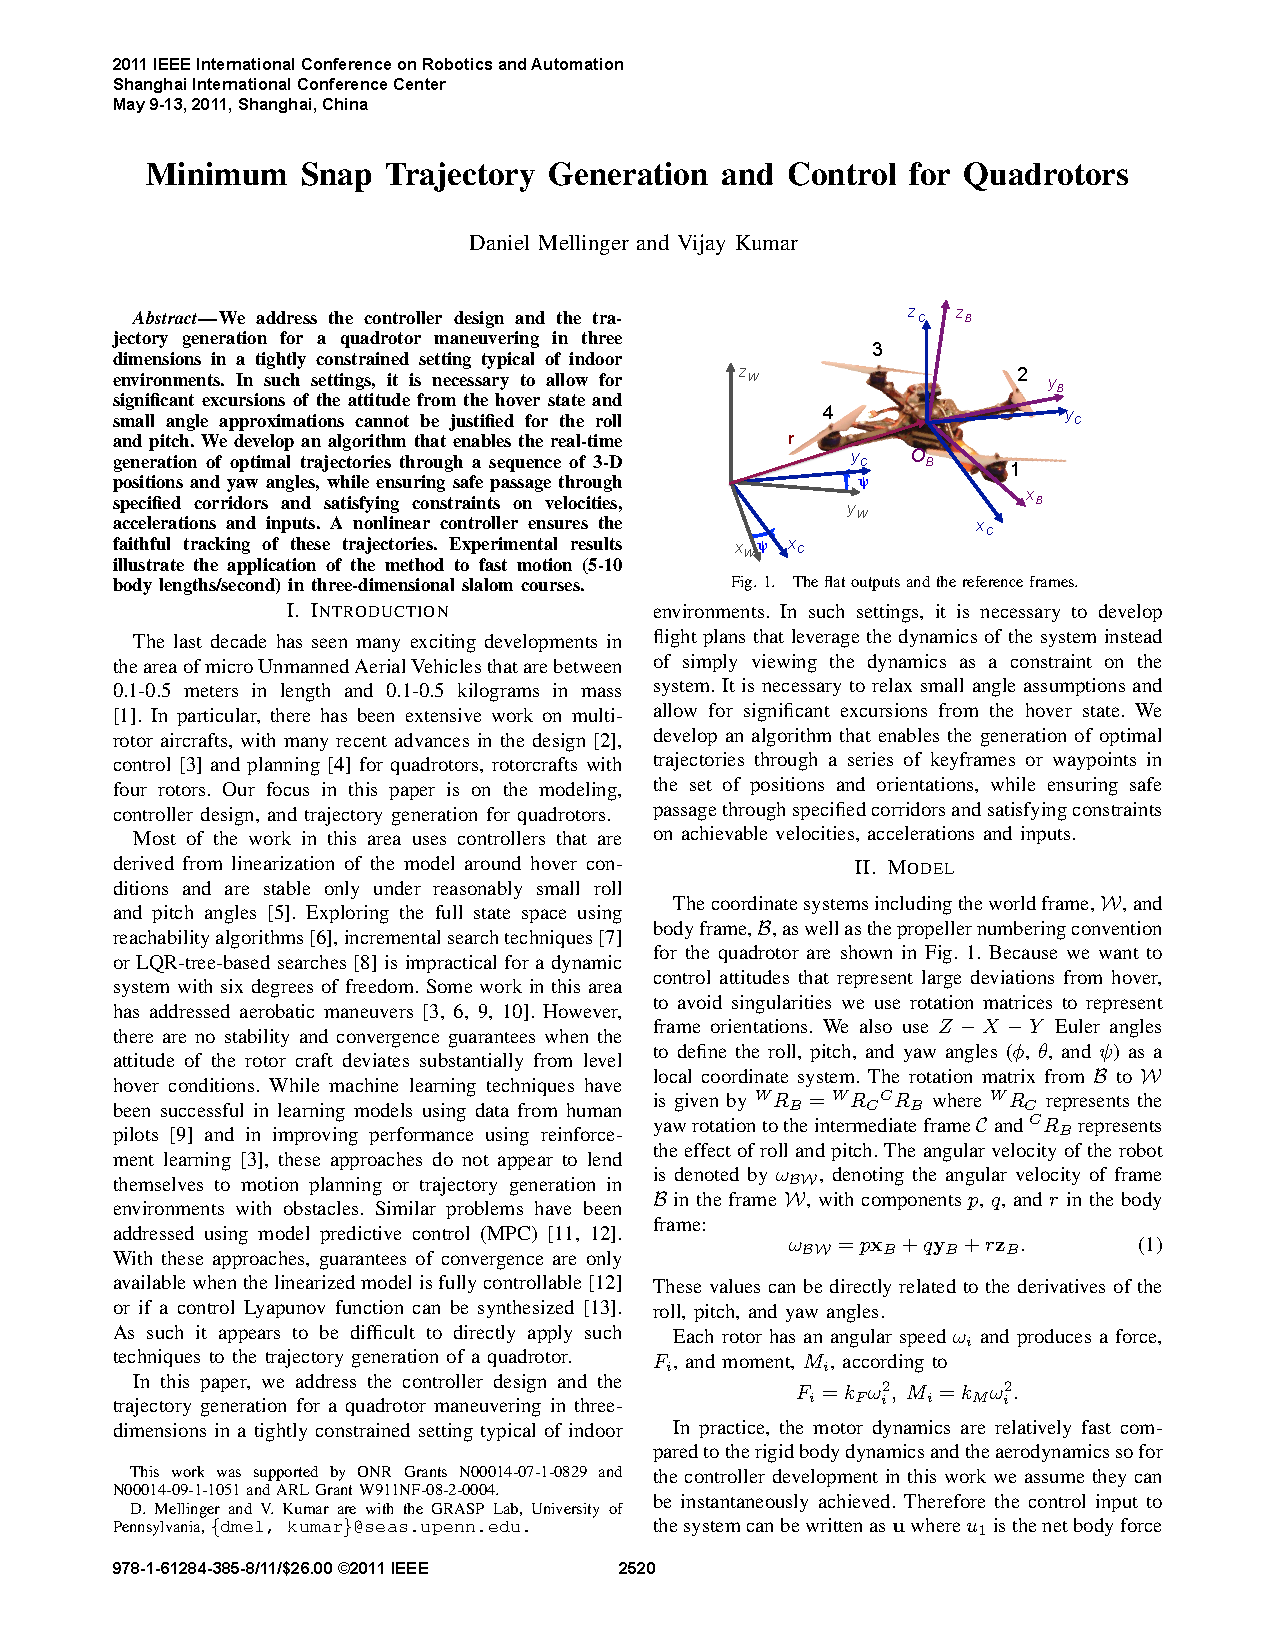
\includepdf[pages=-,scale=.8,pagecommand={}]{chap5_trajectory_planning/papers/MellingerKumar11.pdf}


%----------------------------------
\section{Voxel map}

\rwbcomment{Add Thane's stuff here.}

\subsection{OctoMaps}
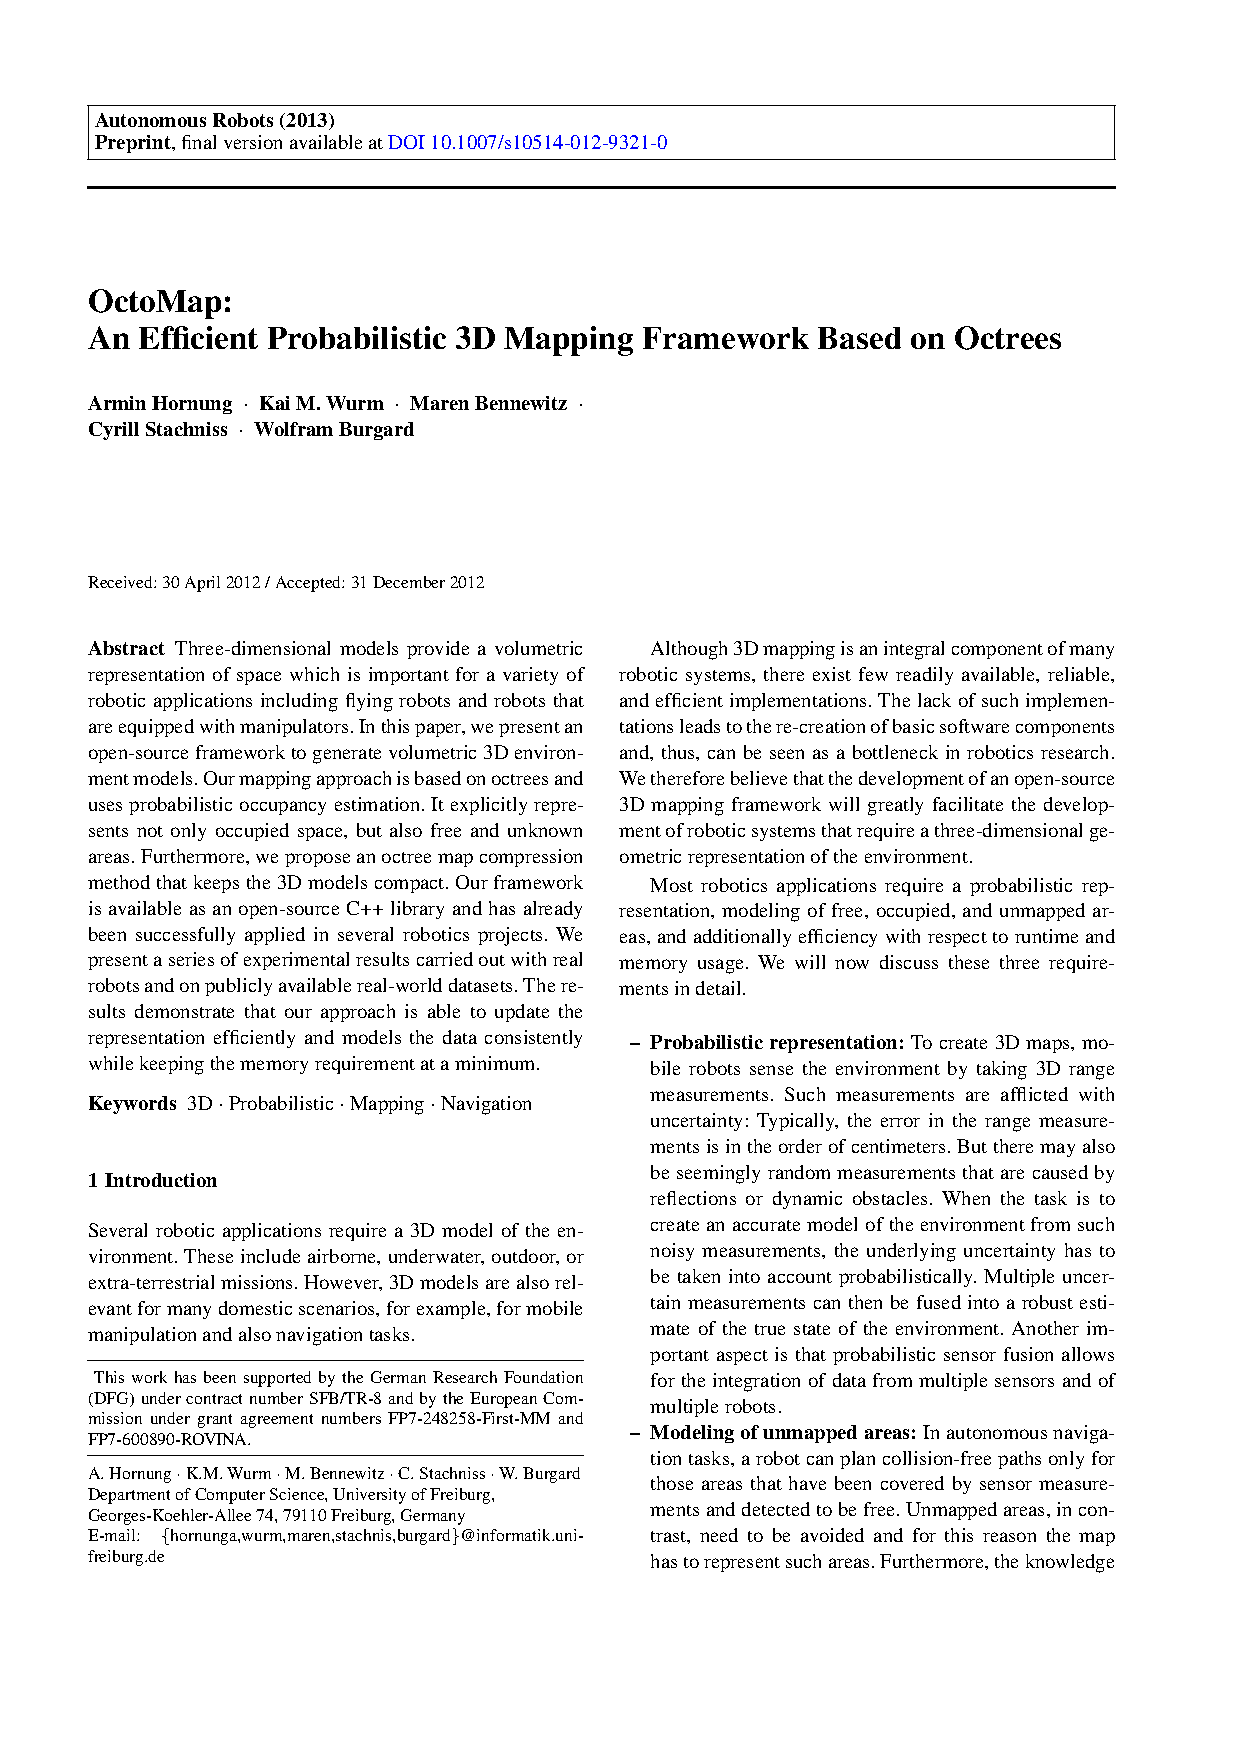
\includepdf[pages=-,scale=.8,pagecommand={}]{chap5_trajectory_planning/papers/Octomap.pdf}


%----------------------------------
\section{Waypoint planning in a voxel map}

\subsection{Graph searching methods}
%
\begin{marginfigure}
  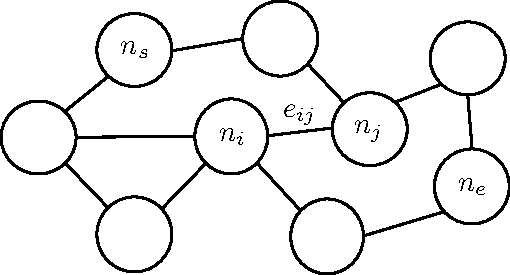
\includegraphics[width=\linewidth]{chap5_trajectory_planning/figures/plan-graph}
  \caption{General graph structure for path planning.}
  \label{fig:plan-graph}  
\end{marginfigure}
%
We can model our world efficiently using discrete graphs where the nodes of the graph represent locations and the edges represent paths between locations. Typically we associate a cost with traveling along an edge from one node to the next. Figure~\ref{fig:plan-graph} shows a simple graph with a start node $n_s$, an end node $n_e$, and intermediate nodes $n_i$ and $n_j$. The cost for traveling along the edge from node $n_i$ to node $n_j$ is given by $e_{ij}$. Although not labeled, each edge has an associated cost. Edges can be unidirectional or bidirectional with with a uniform or different edge cost for each traversal direction. Edge costs can be used to represent proximity to obstacles, the physical distance between the two nodes, or other features of the environment. 

The voxel maps described in the prior section can be represented as a graph structure where the center of the voxel is the node and cost for moving between adjacent voxels is the associated edge cost. To plan paths from a starting location in the voxel map to the specified goal location, we will utilize graph searching methods including widely used approaches such as Djikstra's algorithm and A* search.

\vspace{1.0in}

\rwbcomment{Add something like the following:}

\href{https://www.redblobgames.com/pathfinding/a-star/introduction.html}{Introduction to A*}
\href{https://brilliant.org/wiki/dijkstras-short-path-finder/}{Dijkstra's Algorithm}




